\documentclass[a4paper,11pt]{book}
%\usepackage{ml2k}
%\usepackage{epsf}
%\usepackage{mlapa}
%\usepackage[pdftex, colorlinks=true, citecolor=black, citebordercolor={.99 .99 .99}, linkbordercolor={.99 .99 .99}, pdfborder={0 0 1 [3]}]{hyperref}
\usepackage[pdftex, citebordercolor={.99 .99 .99}, linkbordercolor={.99 .99 .99}, pdfborder={0 0 1 [3]}]{hyperref}

\usepackage[fixlanguage]{babelbib}
\selectbiblanguage{spanish}

\usepackage[spanish, activeacute]{babel}
\selectlanguage{spanish}

% PRINT version
%\setlength{\oddsidemargin}{-20pt}
%\setlength{\evensidemargin}{-20pt}
%\setlength{\marginparwidth}{57pt}
%\setlength{\footskip}{30pt}
%\addtolength{\textwidth}{146pt}

% BOOK version
\setlength{\oddsidemargin}{53pt}
\setlength{\evensidemargin}{53pt}
\setlength{\marginparwidth}{57pt}
\setlength{\footskip}{30pt}


\usepackage[sort]{natbib}
\usepackage{psfrag}
\usepackage{fancyhdr}
\usepackage{appendix}
\usepackage{layout} 
\usepackage{graphicx} % para incluir graficos
\usepackage{amsmath} 
\usepackage{amsthm} % para escribir teoremas lindos
\usepackage{amsfonts} % para tener el simbolo de los numeros reales
\usepackage{color}  % colores de las fuentes

\usepackage{listings} % algoritmos
\lstdefinelanguage{chanfle}{	    
 	 morecomment=[l]{//},
 	 morecomment=[s]{/*}{*/},
   literate={:=}{{$\gets$}}1
   					{<-}{{$\gets$}}1
            {/not}{{$\neg$}}1
            {/and}{{$\land$}}2
            {/andThen}{{$\land_L$}}2
            {/or}{{$\lor$}}2
            {/orThen}{{$\lor_L$}}2
            {/imp}{{$\Rightarrow$}}2
            {/impThen}{{$\Rightarrow_L$}}2
            {/conjVacio}{$\emptyset$}1
            {/alpha}{$\alpha$}1
            {/alfa}{$\alpha$}1
            {->}{$\rightarrow$}2
            {NULL}{\sc{null}}4,
   keywords={if,for,then,else,while,fi,wend,true,false,var,case,of,esac,in,out,inout},
}

\lstnewenvironment{algoritmo}{}{}

\lstset{
	language=chanfle,
	basicstyle=\small,
	flexiblecolumns=false,
	basewidth={0.5em,0.45em},
	keywordstyle=\bfseries,
	tabsize=4
}

% Redefine plain page style
\fancypagestyle{plain}{
\fancyhf{}
\renewcommand{\headrulewidth}{0pt}
\fancyfoot[LE,RO]{\thepage}
}

% Code for creating empty pages
% No headers on empty pages before new chapter
\makeatletter
\def\cleardoublepage{\clearpage\if@twoside \ifodd\c@page\else
    \hbox{}
    \thispagestyle{plain}
    \newpage
    \if@twocolumn\hbox{}\newpage\fi\fi\fi}
\makeatother \clearpage{\pagestyle{plain}\cleardoublepage}

% Define pagestyle
\pagestyle{fancy}
\fancyhf{}
\renewcommand{\chaptermark}[1]{\markboth{ \emph{#1}}{}}
\fancyhead[LO]{}
\fancyhead[RE]{\leftmark}
\fancyfoot[LE,RO]{\thepage}

% Detalle de la TOC
\setcounter{tocdepth}{1}


\theoremstyle{definition} \newtheorem{axiom}{Axioma}
\theoremstyle{theorem} \newtheorem{teorema}{Teorema}

\begin{document}
\bibliographystyle{plainnat}
\bibpunct{(}{)}{,}{a}{,}{,}

\makeatother
\newcommand{\Nat}{\mathbb{N}}
% intervalo melodico
\newcommand{\IM}[1]{\underline{#1}}
\newcommand{\cita}{\textcolor{red}{cita}}
\newcommand{\alert}[1]{\footnote{\textcolor{red}{#1}}}
\newcommand{\red}[1]{\textcolor{red}{#1}}

%\newcommand{\alert}[1]{\textcolor{red}{#1}}
\newcommand{\mycomment}[1]{\textcolor{blue}{#1}\newline}
%\renewcommand{\comment}[1]{\ }
\theoremstyle{definition} \newtheorem{definition}{Definici'on}


\newcommand{\defaultAlignment}{center}
\newcommand{\defaultWidth}{12.5cm}
\newcommand{\defaultPosition}{h}
\newenvironment{imagen}{
\let\File\empty
\let\Desc\empty
\let\LabelName\empty
\let\Width\textwidth
\let\Alignment\defaultAlignment
\let\Position\defaultPosition
}{
    \begin{figure}[\Position]
    \begin{\Alignment}
    \includegraphics[width=\Width]{\File}
    \caption{\Desc}
    \label{\LabelName}
    \end{\Alignment}
    \end{figure}

}

\newcommand{\position}[1]{\def\Position{#1}}
\newcommand{\file}[1]{\def\File{#1}}
\newcommand{\desc}[1]{\def\Desc{#1}}
\newcommand{\labelname}[1]{\def\LabelName{#1}}
\newcommand{\width}[1]{\def\Width{#1}}
\newcommand{\alignment}[1]{\def\Alignment{#1}}


%\begin{abstract}
%asd
%\end{abstract}

\frontmatter

%\title{Hacia una validaci\'on generativa de teor\'ias cognitivas musicales}
\author{Pablo Hern\'an Rodr\'iguez Zivic}
\date{}
\maketitle

\thispagestyle{empty}

\begin {center}

\includegraphics[scale=.3]{uba2.jpg}

\medskip
UNIVERSIDAD DE BUENOS AIRES

Facultad de Ciencias Exactas y Naturales


\vspace{3cm}


\textbf{\Large Hacia una validaci\'on generativa de teor\'ias cognitivas musicales}

\vspace{2cm}



\vspace{2cm}

\textbf{Pablo Hern\'an Rodr\'iguez Zivic}

\end {center}


\vspace{1.5cm}

\noindent Director de tesis: Carlos Diuk

\noindent Co-director: Favio Shifres 


\vspace{1cm}

\vspace{1cm}

\noindent Buenos Aires, 2009



%\section*{Agradecimientos}
La lista de agradecimientos realmente es s'uper larga. Creo que en mayor o menor medida, todos los que estuvieron cerca mio este 'ultimo a~no de alguna forma
aportaron a que ahora s'olo me falte escribir los agradecimientos. \newline

Si bien es verdad que todos los que estuvieron cerca mio en cierta forma me ayudaron, hay varias personas que vale mencionar. \newline

Los primeros son mis queridos viejos: Mam'a y Pap'a, m'as conocidos como Silvia Zivic y Carlos Rodriguez. Estoy muy agradecido de todo el vuelo que me ayudaron a tomar
desde que recuerdo: estoy convencido de que gran parte de todo esto fue gracias a que mi papi me ense~n'o la Ley de Ohm cuando ten'ia unos 7 a~nos, 
y mami me ense~n'o a tocar el piano cuando ten'ia unos 4 a~nitos.\newline

Tambi'en quiero agradecer a los pibe'$\ $ de la facu, no podr'ia haber aprendido todo lo que aprend'i si no fuera por ellos: trabajamos y nos divertimos juajuaja. 
Posta, gracias a PabloB, Lata, el Sabi, Jota, Luigi, la Topa, Piter, Droopy, Toto, Guidh'in, el Roque~no y Eze.\newline

No me olvido de ustedes, no se pongan celosos, tal vez ahora no nos vemos tanto, pero son como mi familia: Noe, Moni, Henry, Armandito, Melu, Ceci, Nati, Adri y 
Gianni. \newline

Jime, te quiero mencionar aparte. Me ayudaste un mont'on en un momento s'uper duro, y gracias a eso pude poner distancia y mirar friamente para darle
un punto final a este trabajo. !`Gracias por estar siempre! \newline

No hay que quitarle m'erito a todos los que padecieron las primeras composiciones de la compositora: si ahora no es placentero escucharla, imaginate antes. 
Esta gente es basicamente la que comparte mi d'ia a d'ia: El Mono, Diego, Santi H., Vic, Manu, Bru, Edu, Cono, Tom, Luiso, Coni, Fer (Zuzuzuzunino!), 
Santi Coffey y Santi Siri.\newline

Mis queridos directores que se bancan mis rayes, mis explociones de mails, mis terquedades, y todas esas cualidades tan lindas con las que tienen que lidiar: 
Gracias Favio!, Gracias Greg!\newline

Adem'as hay que bancarse leer estas 94 p'aginas, !`Gracias a Agust'in y a Pablo por dedicarme ese tiempo!\newline

\begin{center}
\LARGE{!`Gracias!}
\end{center}

%\include{abstract}
%\include{msc_titlepage}
%\include{msc_preface}
%\include{msc_summary}

% Remove parskip for toc
\setlength{\parskip}{0ex plus 0.5ex minus 0.2ex}
\tableofcontents

\mainmatter
% Adjustments headers
\fancyhead[LO]{\leftmark}
\fancyhead[RE]{\emph{Cap\'itulo \thechapter}}


\chapter{Introducci\'on}
\section{Introducci\'on y objetivos}
Hacia fines del siglo XIX y principios del siglo XX (\alert{revisar}), con el prop'osito de estudiar la estructura interna de una pieza musical, 
Heinrich Schenker elabor'o una teor'ia de la coerencia tonal en la m'usica conocido como \texttt{an'alisis schenkeriano}.
En su teor'ia, Schenker postula que la superficie musical (lo que se escucha) es resultado de sucesivas transformaciones que sufre una estructura b'asica fundamental 
denominada por el autor la \emph{ursatz}\footnote{estructura fundamental en alem'an}. Estas transformaci'ones estan descriptas en t'erminos de reglas de reescritura que permiten 
a partir de una cierta ursatz llegar a una pieza musical competa. Dado que la ursatz es la estructura fundamental, 'esta s'olo contiene las notas que dan la impronta de la pieza, 
que luego son elaboradas usando las reglas de reescritura.

Si bien el an'alisis schenkeriano fue concebido para llevar la ursatz a una pieza musical completa, queda claro que se lo puede utilizar tambi'en para estimar
cual podr'ia ser la ursatz de un cierta superficie musical. De esta forma, al utilizar la teor'ia ``en sentido contrario'', en vez de hablar en t'erminos de elaboraci'ones de 
la ursatz a la superficie musical, habr'ia que hacerlo en terminos de reducciones. Definida como lo opuesto a una elaboraci'on, una reducci'on permite especificar que una cierta 
nota dentro de un grupo es la estructuralmente mas importante, y que todo el resto es una \texttt{elaboraci'on} de esta. 
Dado que esta relaci'on de reducci'on/elaboraci'on se puede aplicar recursivamente, naturalmente emerge una relaci'on 
jer'arquica entre las notas de una pieza musical.  En esta jerarqu'ia, el nivel m'as bajo es lo que se encuentra escrito en la partitura, y a medida que se sube de nivel se 
encuentra la misma pieza musical, pero carente de elaboraciones. En la figura \ref{fig_analisis_schenkeriano} se exhibe un ejemplo de dicho an'alisis.


\begin{figure}[h]
\begin{center}
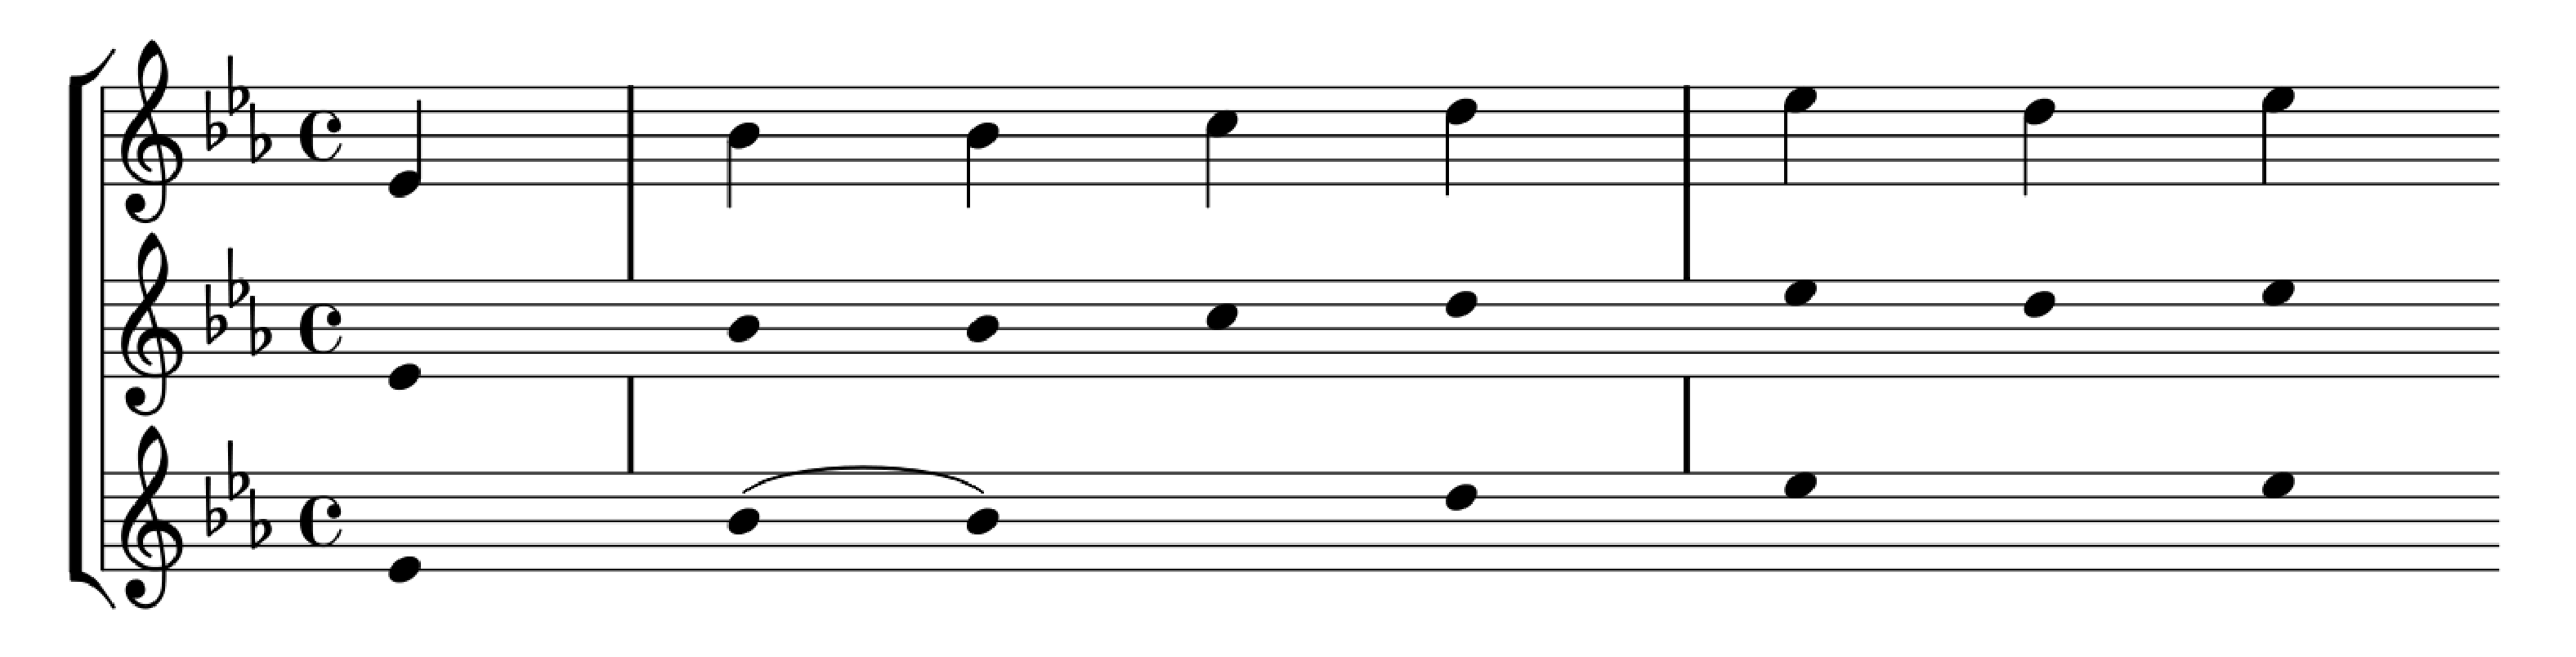
\includegraphics[width=12cm]{images/schenkerian_example}
\label{fig_analisis_schenkeriano}
\newline \alert{poner una imagen mas copada}
\end{center}
\end{figure}

En esta figura, los sucesivos pentagramas muestran relaciones de reducci'on, as'i simplificando el tema con el objeto de llevarlo a una representaci'on m'as abstracta.

El parecido de este tipo de relaciones con las relaci'ones utilizadas por Noam Chomsky para analizar el lenguaje natural es notable. 
Si bien en la teor'ia de Chomsky las relaciones son relaciones del tipo ``es un'', y en la teor'ia de Schenker son del tipo ``es una elaboraci'on de'', 
estas se enmarcan matem'aticamente en el mismo lugar.  

En 1983, el m'usico Fred Lerdahl y el ling\"uista Ray Jackendoff publicaron el libro 
\texttt{A Generative Theory of Tonal Music}(GTTM) donde proponen una gram'atica para analizar la m'usica t'erminos parecidos a los de Schenker. 
Lo interesante de este trabajo es el fundamento que se le da a la elecci'on de las reglas de la gram'atica, puesto que proponen una teor'ia que tomando los conceptos claves
de la teor'ia schenkeriana se basa en supuestos cognitivos de naturaleza computacional.

El objetivo del trabajo de Lerdahl y Jackendoff es principalmente tener modelizar el proceso mediante el cual se estructura la percepci'on de la m'usica. 
Este modelo consiste en una serie de reglas de preferencia. Cada regla tiene asociado un predicado booleano $P$ y un valor de preferencia $v$, 
de modo que si el predicado booleano es verdadero, entonces aportan $v$ unidades a la preferencia de una cierta acci'on interpretativa. Para ejemplificar, a continuaci'on se cita
una regla de preferencia de los autores. Esta regla es una de las reglas asociadas a lo que los autores llaman agrupamiento, que b'asicamente consiste en agrupar notas que tienen
significancia de frase\footnote{M'as adelante se explicar'a esto con mayor detalle}.
\newline

\begin{center}
\texttt{GPR 1} Evite fuertemente grupos que contengan solamente un evento.
\end{center}

En este caso, el predicado booleano es aquel que es verdadero solamente con grupos de cardinalidad uno, y el valor de preferencia es fuertemente negativo a la acci'on interpretativa
de decidir que el grupo en cuesti'on debe contener 'unicamente al evento que contiene. 

Si bien un modelo de este tipo es generativo en el sentido de que podr'ia ser utilizado por una computadora tanto para analizar una pieza musical como para 
\texttt{generar} una nueva, es importante notar que este no es su objetivo. 
Puede verse claramente como la regla \emph{GPR 1} si bien es suficientemente rigurosa como para luego poder corroborarla emp'iricamente, no lo es como para construir un 
programa que haga un an'alisis utilizando esta regla: es necesario determinar el valor de preferencia y aprender las relaci'ones entre los distintos valores de preferencia para luego 
tomar una desici'on.  

De esta forma se discrimina entre \texttt{modelos generativos}, que son aquellos que eventualmente podr'ian utilizarse para generar aquello que explican, y 
\texttt{modelos de 'indole generativo} que fueron hechos con el objeto de generar aquello que explican.  El hecho de que sea necesario definir expl'icitamente los valores de preferencias
sumado a que este modelo no es de 'indole generativo plantea el interrogante de si realmente este enfoque es el adecuado para para modelar la cognici'on musical con aprendizaje 
autom'atico. 

De este modo, el objetivo de este trabajo es utilizar el conocimiento generado por trabajos como el de Lerdahl y Jackendoff como medio para establecer propiedades que un modelo de 
'indole generativo deber'ia cumplir. Teniendo estas propiedades, luego es posible construir un modelo desvinculado de la idea de gram'atica, que respete 
ciertos criterios fundamentales. Si se logra conseguir un modelo de estas caracter'isticas se podr'an validar emp'iricamente los criterios en base a los que el modelo fue construido 
(y por lo tanto las teor'ias cognitivas que motivaron los criterios) a trav'es de analizar las piezas musicales generadas por el modelo.

Para poder avanzar en pos del objetivo recien planteado, es necesario primero sentar un vocabulario para luego poder contextualizarlo. De esta forma, las siguientes dos
secci'ones hablaran sobre background. Luego se har'a un breve resumen sobre el estado del arte en este tema, para luego abordar el trabajo en concreto de esta tesis.


\section{Estado del arte}
A continuaci'on se har'a un breve resumen sobre los distintos enfoques y objetivos relacionados con el an'alisis musical mediante
t'ecnicas computacionales. Las aplicaciones de este tipo de trabajos son bastante variadas, tales como herramientas para 
composici'on musical asistida, acompa~namiento autom'atico, indexaci'on de m'usica, sistemas de recomendaci'on musical e 
investigaci'on en psicolog'ia de la m'usica, donde se situa este trabajo.

Seg'un cual sea el enfoque que se tome, podr'a variar la representaci'on musical utilizada entre la se~nal sonora cruda, y una partitura o midi.
En este trabajo se asumir'a una representaci'on simb'olica de la m'usica para poder desarrollar en profundidad las teor'ias cognitivas de las 
que luego se hablar'a. A continuaci'on se nombran algunos trabajos que se enmarcan de la misma forma en t'erminos de la representaci'on musical.

\cite{PaieThesis} es el trabajo m'as cercano a 'este. En 'el se propone un modelo generativo para l'ineas mel'odicas, 
patrones r'itmicos y armonizaci'ones, basado en algunos de los principios que se utilizar'an en este trabajo. 
Sin embargo, no es el objetivo del autor poner a prueba teor'ias cognitivas de la m'usica; sino desarrollar un modelo generativo,
y por lo tanto predictivo basado en una representaci'on simb'olica de la m'usica de forma tal que se pueda utilizar el conocimiento generado por estos
modelos para mejorar la calidad de algoritmos que trabajan con se~nales sonoras. M'as all'a de que no se comparten los objetivos entre el trabajo de 
Paiement y este, no es posible tampoco utilizar los modelos propuestos por 'el puesto hay teor'ias que no utiliza, como la de \citealp{Lerdahl2001} 
y varios de ellos, como el de la r'itmica, no tienen una fundamentaci'on cognitiva clara.

David Cope, en \cita trabaja con un software, que mediante reglas, sea capaz de reproducir el estilo de una pieza musical dada. Si bien 
la construcci'on ha sido exitosa en algunos casos, generando composiciones que realmente respetan el estilo de la pieza original, gran
parte de las reglas utilizadas no tienen sustento cognitivo.

Otro software existente dise~nado para componer m'usica es el Melisma Music Generator
\footnote{Disponible en http://www.link.cs.cmu.edu/melody-generator/} basado en \cite{Temperley2004}. 
Este software se encuentra disponible para escuchar online sus composiciones, sin embargo, el mayor problema 
que tiene es que no se puede entrenar directamente con su modelo con una partitura, y por m'as que se intentara realizar esto construyendo un software 
que estime valores posibles para sus par'ametros, no habr'ia forma de determinarle una sucesi'on de contextos arm'onicos.

\red{revisar bien si no estoy diciendo verdura}
\cite{Shih-Chuan} propone un software que mediante la utilizaci'on de t'ecnicas de data minning componga m'usica. Nuevamente, estos modelos
no son de intere'es para este trabajo puesto que pr'acticamente no tienen ning'un fundamento cognitivo, y siendo asi, no podr'a realizarse 
ning'un tipo de validaci'on.
%
%En \cite{Simon_mysong:automatic} mediante el an'alisis de caracter'isticas de la se~nal sonora correspondientes a una melod'ia 
%cantada, y mediante entrenar un Hidden Markov Model para la probabilidad de un acorde, dado que se observa una cierta nota cantada,
%se construy'o un sistema capaz de armonizar una melod'ia. Un sistema comercial que realiza esto mismo es Band-in-a-box,
%pero dado que no existen \red{revisar} publicaciones respecto a c'omo fue construido, no se puede hacer m'as que nombrarlo.
%
%Dentro de la rama de sistemas para indexar m'usica se situan trabajos como \cite{StructureAnalysis1}. En 
%\cite{StructureAnalysis1} se propone un m'etodo para analizar la estructura de una pieza musical a partir de su se~nal sonora. Esto lo logran extrayendo vectores 12-dimencionales
%de cada momento del tema, en donde cada componente del vector muestra la intencidad relativa de cada altura en ese momento, y a partir
%de estos vectores y una noci'on de distancia construyen matrices de similitud que permiten detectar los acordes que aparecen
%en el tema. Siguiendo con este 

\section{Aportes de este trabajo}

\chapter{Background}
\label{cap:background}
\section{Notas, alturas, acordes y tonalidades}
\label{sec:musical_intro}
Esta secci'on cumple dos objetivos dentro de este trabajo; por un lado, sirve para el lector no familiarizado con teor'ia musical para establecer
ciertos conceptos generales que son de gran importancia en el desarrollo de este trabajo. Por otro lado, permitir'a adem'as acentar un glosario
que se utilizar'a a lo largo de las diferentes secciones.

Principalmente, la m'usica tonal se divide en dos grandes componentes u ejes: la del \texttt{tiempo} y la de la \texttt{altura}. 

La dimensi'on temporal responde a \emph{cu'ando} ocurre un evento, mientras que la altura expresa caracter'isticas sobre \emph{qu'e}
tipo de evento es.  Dejando fuera del an'alisis a los instrumentos de percusi'on, la altura es refiere a la percepci'on de un cierto sonido. 
Esta percepci'on si bien esta relacionada con caracter'isticas intr'insecas del sonido, como su intensidad, timbre y frecuencia, 
tambi'en hace referencia
al proceso cognitivo que ocurre por parte del oyente. De esta forma, si bien un sonido de una frecuencia de $440Hz$ es percibido como una nota 
$La$, tambi'en lo es un sonido de frecuencia $441Hz$.

Dentro de la m'usica occidental, existen criterios dentro de ambas componentes que ayudan a la organizaci'on de una pieza musical. 
En lo subsiguiente se introducir'an ciertos conceptos de la teor'ia musical, puesto que son necesarios
para abordar los fundamentos cognitivos y los modelos propuestos. 

Por 'ultimo, dado que a lo largo del presente trabajo se exhiben ejemplos, es necesario que el lector sepa comprender una partitura sencilla, de forma que se se 
explicar'a brevemente como ciertos conceptos introducidos se notan en el lenguaje musical.

\subsection{Sobre la organizaci\'on temporal}
El primer concepto importante a tener en cuenta, es que el tiempo es \emph{discreto}. Esto no quiere decir que a la hora de la producci'on musical lo sea, sino que 
en la abstracci'on musical, existe una unidad de referencia temporal, a la que se llama \emph{beat}. En torno a ella se organiza la estructura temporal, tocando
siempre notas que duren una fracci'on del mismo. De esta forma, para poder reproducir una partitura es necesario saber la duraci'on de un \emph{beat} (denominado
\emph{tempo}), luego el resto de las duraciones son una fracci'on de 'esta.


En su libro, \citet*{LerdahlJackendoff83} hacen una distinci'on entre dos estructuras que ocurren en simultaneidad en la m'usica tonal:
La estructura \emph{m'etrica} y la estructura del \emph{agrupamiento}\footnote{\emph{meter} y \emph{grouping} en ingl'es}. 
Esta distinci'on en t'erminos generales coincide con clasificaciones de otros autores (\alert{citas muchas!}), se toma la version de Lerdahl y Jackendoff 
por ser esta m'as computacional.
La estructura del agrupamiento hace referencia a la organizaci'on de una pieza musical en unidades que pueden ser motivos, frases, secciones, etc. 
Cada una de estas unidades, es denominada por los autores como \emph{grupo}. Asimismo, el oyente infiere una estructura regular de beats. 
Algunos beats reciben una acentuaci'on mayor que otros, determinando lo que los autores definen como la estructura m'etrica. Dentro de esta estructura
existen distintos niveles, cada uno determinado por el tiempo transcurrido entre dos beats consecutivos. 
Un nivel posible es el llamado \emph{tactus} que corresponde de alguna forma al \emph{beat principal del tema}\footnote{Cognition of basic musical structures, p'agina 52}.
Se referir'a por contexto m'etrico de una pieza a la estructura m'etrica que se infiere a partir de esta.

Ambas estructuras son jer'arquicas, en el sentido de que existen sub-estructuras a distintos niveles, y que las sub-estructuras de niveles superiores 
incluyen por completo a las de nivel inferior
\footnote{Para una definici'on m'as formal de la jerarqu'ia referirse a \cite[p. XXX]{LerdahlJackendoff83}}. De esta forma, una secci'on
de una pieza musical estar'a formada por una sucesi'on de frases. Estas frases s'olo pertenecer'an a esa secci'on, sin embargo, esto no quiere decir
que no se pueda repetir una frase en dos secciones distitnas, puesto que cada una pertenecer'a a una sola secci'on. 

%\red{este parrafo no est'a bien, lo dejo para acordarme de reescribirlo}
%
%La organizaci'on jer'arquica de la m'usica no es una teor'ia solo postulada por Lerdahl y Jackendoff; Cooper y Meyer (\cite{CooperMeyer60}) plantean una teor'ia similar en
%estos t'erminos, Kramer (\cite{Kramer88}) si bien no habla directamente de una jerarqu'ia, propone que tienen un rol 
%estructurante\alert{tengo que leer m'as, as'i se mejor de lo que hablan estos dos muchachos}. 
%
%Un nivel de especial inter'es, es el denominado \emph{tactus}, que b'asicamente es el marcado por el director de orquesta al mover su batuta. 
%El tactus tambi'en es la distancia entre los beats que el oyente marca cuando mueve el pie y est'a relacionado con el baile. 
%
Es importante notar que esta estructura es ambigua, en el sentido de que que muchas veces no existe un 'unico an'alisis de una pieza musical 
en una estructura m'etrica y de agrupamiento.


Retomando con la duraci'on de las notas, dado que cada nota no puede tener una duraci'on arbitraria, y que esta duraci'on est'a relacionada con el tempo
a trav'es de una fracci'on, existen s'imbolos y nombres para diferentes duraci'ones. 
En la figura \ref{fig:durations} se muestran las figuras correspondientes a notas y silencios de distintas duraciones. Se denomina plica, a la barra vertical que surje 
de la cabeza de las notas, con excepcion de la redonda. Es importante aclarar que cuando dos notas de duracion inferior o igual a una corchea se tocan juntas, 
se unen las plicas, m'as adelante se dar'a un ejemplo.

\begin{imagen}
    \file{images/figures.png}
    \labelname{fig:durations}
    \desc{Figuras de ejemplo}
    \width{12cm}
\end{imagen}

Las partituras luego se organizan en una serie de unidades, cada una denominada \emph{comp'as}. Todos los compases tienen la misma duraci'on, y esta se especifica
en la partitura por una fracci'on al comienzo de la misma. Esta fracci'on no debe interpretar de forma usual, ya que posee una sem'antica sutilmente diferente.
En la especificaci'on del comp'as, el denominador determina en que unidades se medir'a la longitud del comp'as, y el numerador determina cuantas unidades 
este durar'a. El valor de referencia para el denominador es el $4$ refiriendo a una negra, y m'ultiplos de este refieren a m'ultiplos de una negra. Por ejemplo
$8$ refiere a corcheas.  De esta forma, un comp'as de $\frac{3}{4}$ indica que la unidad de referencia es la negra, y que hay $3$ negras por comp'as.
La figura \ref{fig:time_signatures} muestra los compases m'as comunes. 

\begin{imagen}
    \file{images/Common_time_signatures.png}
    \labelname{fig:time_signatures}
    \desc{Compases comunes}
    \width{5cm}
\end{imagen}

Observar que a fines de notar la duraci'on del comp'as, no existe diferencia entre el comp'as de $\frac{3}{4}$ y el comp'as de $\frac{6}{8}$, su diferencia
radica en la acentuaci'on recibida por distintos eventos: En el comp'as de $\frac{3}{4}$, existen 3 eventos de negra, donde el primero se percibe como acentuado, 
y los dos siguientes se perciben con una acentuaci'on m'as d'ebil, mientras que en el comp'as de $\frac{6}{8}$ hay 6 eventos, donde el primero es el m'as 
acentuado, luego sigue el cuarto, y por ultimo el resto de los beats.

Adem'as de los s'imbolos explicados, existen ciertos s'imbolos que permiten que el lenguaje sea m'as rico, y describir nuevas duraciones. La ligadura
permite sumar la duraci'on de dos figuras. Un caso particular de la ligadura, es el puntillo. El puntillo se nota como un peque~no punto que se coloca a 
continuaci'on de la cabeza de una nota, y determina que la duraci'on de esa nota debe multiplicarse por $\frac{3}{2}$. 
De esta forma, una \emph{negra con puntillo}, dura una negra y media. 

Para fijar conceptos, se exhibe una partitura de ejemplo en la figura \ref{fig:example_measure}. 
La duraci'on del primer s'imbolo es $\frac{3}{4}=\frac{1}{2}\times\frac{3}{2}$,
la duraci'on del segundo s'imbolo es $\frac{1}{4}$, puesto que tiene dos plicas, y eso indica que es una semicorchea. Luego sigue un silencio de negra,
y una negra ligada a una semi corchea, es decir, su duracion sera $1 + \frac{1}{4}$, luego sigue una semi corchea y un silencio de corchea, completando
con la duraci'on total de 4 negras. La letra $c$ al principio del comp'as es una abreviaci'on para decir $\frac{4}{4}$.

\begin{imagen}
    \file{images/pedagogic_measure.png}
    \labelname{fig:example_measure}
    \desc{Ejemplo para fijar conceptos}
    \width{12.5cm}
\end{imagen}

\subsection{Sobre la organizaci\'on de las alturas}
La m'usica tonal refiere a m'usica donde una altura funciona como punto de referencia. Este punto de referencia es una nota llamada t'onica y es
la que le da nombre a la escala; por ejemplo Do es la t'onica de la escala de Do mayor. 

Existen dos formas alternativas de denominar a las notas, la usual que utiliza los nombres Do, Re, Mi, Fa, Sol, La y Si y la americana, que 
asigna letras a cada nota resultando en C, D, F, E, G, A y B respectivamente. Se utilizar'an ambas formas para referirse a las notas de forma
intercambiable. 

Continuando con las escalas, las escalas mayores y menores de la m'usica occidental, llamadas escalas diat'onicas, 
son un subconjunto de siete alturas de la escala crom'atica.
La escala crom'atica es aquella que divide, sobre una escala logar'itmica, en 12 partes iguales a las frecuencias cuya raz'on es 2. Por ejemplo, 
la frecuencia de la nota $A$ es $440Hz$. En la tabla \ref{tab:cromatica} se exhibe las frecuencias de las notas de la escala crom'atica 
comenzando desde $A$.

\begin{table}[h]
\begin{center}
\begin{tabular}[c]{|l|c|}
\hline
\textbf{Nota} & \textbf{Frecuencia en $Hz$} \\
\hline 
A		&	440.00 \\
A\#		&	466.16 \\
B		&	493.88 \\
C		&	523.25 \\
C\#		&	554.37 \\
D		&	587.33 \\
D\#		&	622.25 \\
E		&	659.26 \\
F		&	698.46 \\
F\#		&	739.99 \\
G		&	783.99 \\
G\#		&	830.61 \\
A		&	880.00 \\ 
\hline
\end{tabular}
\label{tab:cromatica} 
\end{center}
\end{table}


Utilizando la escala crom'atica se puede definir la noci'on de \emph{semitono} y de \emph{intervalo mel'odico}. Un semitono es la distancia
entre dos notas consecutivas dentro de la escala crom'atica. Por ejemplo $E$ y $F$ est'an a un semitono de distancia. Un intervalo mel'odico, 
es la distancia entre dos notas medida en semitonos .Dentro de la teor'ia musical, a estos intervalos se les pone un nombre que permite \red{>qu'e permite?}. 
Como a lo largo de este trabajo no se utilizaran los nombres de los intervalos mel'odicos, se los nombrar'a como la cantidad de semitonos que separa
a las notas que lo conforman. Por ejemplo, las notas $A$ y $B$ est'an a 2 semitonos de distancia, por lo que el intervalo mel'odico
se notar'a como \IM{2}. 

Como se mencion'o al principio de esta secci'on, de la escala crom'atica se elije un subconjunto de 7 notas. Estas notas ser'an referenciadas
respecto de una nota normativa. El tipo de escala con la que se est'e trabajando depender'a del patr'on de intervalos que forman las 7 notas elegidas
respecto de la t'onica. Por ejemplo, la escala mayor forma el siguiente patr'on:

\begin{center}
\IM{2} \IM{4} \IM{5} \IM{7} \IM{9} \IM{11} \IM{12}
\end{center}

Si se observa el intervalo que forma cada nota respecto de la anterior, el patr'on resultante es el siguiente

\begin{center}
\IM{2} \IM{2} \IM{1} \IM{2} \IM{2} \IM{2} \IM{1}
\end{center}

Si se rota este patr'on un lugar hacia la izquierda, se obtiene el patr'on que forman las escalas menores:

\begin{center}
\IM{2} \IM{1} \IM{2} \IM{2} \IM{2} \IM{1} \IM{2} 
\end{center}

De esta forma, la escala mayor de C estar'a formada por las notas C, D, E, F, G, A, B, mientras que la escala menor de C estar'a formada
por las notas C, D, D\#, F, G, G\#, A\#, B\footnote{Por cuestiones de claridad se escribe la escala de esta forma. La forma correcta
de escribirlo es C, D, Eb, F, G, Ab, Bb, ya que cada nota debe aparecer solo una vez. Se entiende que este detalle es irrelevante a los efectos
de lo que se desea transmitir}


Por 'ultimo, la entidad restante a hacer mensi'on es el \emph{acorde}. Un acorde est'a formado por tres o m'as notas. Cada acorde abarca una regi'on
en el tema, y dentro de la regi'on de dominancia ser'a el foco arm'onico.

Tornando el foco a la lectura musical, existen dos elementos que permiten notar de significado las l'ineas y espacios del pentagrama: la clave
y la armadura de clave. La clave asigna una nota a un rengl'on en particular, y la armadura permite especificar en que escala se tocar'a. 
Dado que a lo largo de este trabajo solo se dar'an ejemplos sobre la tonalidad mayor, se obviar'a la explicaci'on de que es la armadura de clave. 
La clave utilizada para todos los ejemplos de esta tesis ser'a la clave de sol que determina que la segunda l'inea, contando de abajo hacia
arriba, ser'a la nota G. El espacio entre esta l'inea y la siguiente, ser'a la nota A, y as'i sucesivamente. Si se deseara especificar
la nota A\#, basta con anteponer el s'imbolo \# a la cabeza de la nota. En la figura \label{fig:escala_mayor} se exibe la escala de C mayor.


\begin{imagen}
    \file{images/major_scale.png}
    \labelname{fig:escala_mayor}
    \desc{Escala mayor de C}
    \width{12cm}
\end{imagen}


\section{Background matem\'atico}
\subsection{Sobre estad\'istica bayesiana}
Una de las desiciones sobre el alcance de este trabajo es que los modelos construidos ser'an entrenados s'olo con un tema de por vez. 
Esta decisi'on evita el problema de tener que combinar la informaci'on proporcionada por varias piezas musicales, sin embargo, el precio que debe pagarse 
es que para muchos modelos de los que se expondr'an no alcanza solamente con entrenar con una pieza musical, puesto que ciertas estimaciones no ser'ian estad'isticamente 
significativas. 

Una soluci'on a este problema es adoptar una postura bayesiana y tener una creencia previa sobre las caracter'isticas del fen'omeno a modelar, 
y luego actualizar esta creencia previa con la evidencia observada. De esta forma, si el modelo esta basado en una teor'ia cognitiva, se puede utilizar
como creencia previa alg'un estudio donde se haya puesto a prueba esta teor'ia. 

Otra raz'on para utilizar creencias previas es para estimar distribuci'ones de probabilidades suaves, en el sentido de que no asignen valor $0$ a un evento 
por el s'olo hecho de no haberlo observado en la etapa de entrenamiento. Esta propiedad ser'a utilizada para el trabajo con contextos arm'onicos.

Escribiendo esto matem'aticamente, sup'ongase que se cuenta con un modelo parametrizado por un vector $\theta$. 
La creencia previa sobre el fen'omeno a modelar, b'asicamente estar'ia restringiendo \emph{a priori} que tipo de par'ametros son mas probables que otros, 
de esta forma, esta informaci'on se codifica como una distribuci'on de probabilidades sobre $\theta$, $P(\theta)$. 

De esta forma, sup'ongase ahora que se cuenta con cierta evidencia de entrenamiento $x_1,\cdots,x_n$. Al entrenar el modelo, uno quisiera combinar la 
creencia previa dada por $P(\theta)$ junto con la evidencia dada por $x_1,\cdots,x_n$ en una distribuci'on \emph{a posteriori} sobre los par'ametros.
Utilizando la ley de Bayes y la ley de probabilidad total, es posible reescribir la distribuci'on a posteriori de $\theta$ en funci'on de su creencia previa y 
la probabilidad de la observaci'on:

\begin{align}
P(\theta|x_1,\cdots,x_n) &= \frac{P(x_1,\cdots,x_n|\theta) P(\theta)}{P(x_1,\cdots,x_n)} \\
                         &= \frac{P(x_1,\cdots,x_n|\theta) P(\theta)}{\int_\theta{P(x_1,\cdots,x_n|\theta)P(\theta)\mathrm{d}\theta}}
\end{align}

Utilizando ahora la creencia a posteriori sobre $\theta$, la probabilidad de una nueva observaci'on $x$ est'a dada por

$$P(x|x_1,\cdots,x_n) = \int_\theta{P(x|\theta)P(\theta|x_1,\cdots,x_n)}$$

Notar que el resultado de hacer esto elimina el par'ametro $\theta$ como valor, y se utilizan todos los valores posibles asociados a la creencia de que efectivamente
sea ese el valor que parametriza a la distribuci'on que genera las obervaciones.


Un principal problema al aplicar estas t'ecnicas es la resoluci'on de las integrales sobre el espacio de par'ametros, que suele ser multidimensional. 
Sin embargo, hay casos en donde se conocen expresiones anal'iticas para la probabilidad a posteriori de los par'ametros, y en ese caso, se puede utilizar
como p'arametro $E(\theta|x_1,\cdots,x_n)$, \alert{argumentar bien, montacarlo de la intergral converje a la esperanza}.

Un caso conocido es cuando se modelan los datos como provenientes de una distribuci'on multinomial. En este caso, si se codifica la creencia previa
sobre $\theta$ como una distribucion Dirichlet, se puede calcular de una forma muy facil la distribuci'on a posteriori de $\theta$ dado por la siguiente
f'ormula:

\alert{usar delta de dirac}

\begin{align}
    \theta \sim Dirichlet(\alpha_1,\cdots,\alpha_k) \Rightarrow \theta|x_1,\cdots,x_n \sim Dirichet(\alpha_1+n_1,\cdots,\alpha_k+n_k)
\end{align}

Donde los valores $x_i$ pueden tomar uno de $k$ valores posibles, y $n_j$ es la cantidad de veces que se observ'o el j-'esimo valor. 

Utilizando esta f'ormula es posible calcular anal'iticamente la distribuci'on a posteriori de la observaci'on, y luego tomar la esperanza dada por

$$E(\theta|x_1,\cdots,x_n)=\frac{\alpha_i + n_i}{\sum_{j=1}^{k}{\alpha_j+n_j}}$$

%
%\subsection{Combinaci\'ones de distribuci\'ones de probabilidad}
%Una operaci'on muy frecuentemente utilizada a lo largo del presente trabajo es la \texttt{combinaci'on convexa} entre distribuciones
%de probabilidad.
%
%Dadas $p$ y $q$, dos distribuci'ones de probabilidad sobre el conjunto $S$, y un n'umero $0 \leq \alpha \leq 1$, 
%se nota $p +_\alpha q$ a la combinaci'on convexa entre $p$ y $q$, y se define:
%$$(p +_\alpha q)(A) = \alpha \times p(A) + (1-\alpha) \times q(A)$$ 
%
%En caso de referirse a $p+q$, se asume que $\alpha = 1/2$. 
%\newline \newline
%Observaci'ones:
%\begin{itemize}
% \item Se puede demostrar que el resultado de combinar dos distribuci'ones de probabilidad de esta forma es tambi'en una distribuci'on 
%de probabilidad.
%
% \item Notar que esta definici'on puede extenderse para $n$ distribuci'ones de probabilidad. En ese caso se necesitar'an valores 
%$\alpha_1, \dots, \alpha_n$, tales que $\sum_i \alpha_i = 1$. En general, se utilizara $\alpha_i = 1/n$ salvo que se aclare lo contrario.
%\end{itemize}
%

\subsection{Cadenas de Markov}
Supongamos que se desea modelar la evoluci'on de un sistema con respecto al tiempo. Es de esperarse que 
el estado en el que se encuentra el sistema en cierto momento de alguna forma tenga que ver con la historia por la que este transit'o
previamente. 

Las cadenas de Markov de orden $k$ permiten modelar este tipo de dependencias haciendo una asunci'on: la probabilidad de que el sistema vaya a un cierto estado
dado la historia de estados por los que transit'o solo depende en un momento dado \emph{s'olo} depende de los 'ultimos $k$ estados anteriores en los que este transit'o. 
Esta asunci'on es conocida como la propiedad de Markov. 

Formalmente, una cadena de Markov de orden $k$ es una tripla $<S,P>$, donde $S$ es el conjunto de posibles estados del sistema, y $P$ la 
distribuci'on de transici'on, es decir, dados $s_1, \cdots, s_{k+1} \in S$, el valor de $P(s_{k+1} | s_1, \cdots, s_k)$ indica la probabilidad
de que el sistema pase estado $s_{k+1}$ dado que a transitado por los estados $s_1, \cdots, s_k$. 
Volviendo a la propiedad de falta de memoria, ahora es posible expresarla formalmente: $$P(s_{n+1}|s_1,\cdots,s_n) = P(s_{n+1} | s_{n-k}, \cdots, s_n)$$

A modo ilustrativo, sup'ongase que se desea modelar el clima con una cadena de Markov de orden 1, restringiendo el clima a si llueve o no. Siendo asi, el conjunto 
$S$ de estados ser'a $\{llueve, no\ llueve\}$. 

Asumiendo que las probabilidades de transici'on son las dadas en la siguiente tabla, el sistema gr'aficamente se ver'ia como la figura \ref{fig:markov_clima}

\begin{center}
\label{tabla_markov}
\begin{tabular}{l l l l}
$P(lluvia | lluvia) $ & $=0.9$ & $P(lluvia | no\ llueve) $& $=0.1$\\
$P(no\ lluvia | lluvia)  $ & $=0.3$ & $P(no\ lluvia | no\ llueve) $ & $=0.7$\\
\end{tabular}
\end{center}

\begin{imagen}
    \file{images/weather_graph.png}
    \labelname{fig:markov_clima}
    \desc{Representaci'on gr'afica de la cadena de Markov}
    \width{5cm}
\end{imagen}




\chapter{Modelos nota a nota}
\label{cap:notenote}
El presente cap'itulo agrupa una serie de modelos que trabajan mayormente sobre caracter'isticas locales de la cognici'on musical, presentando un modelo 
para generar la r'itmica y otro para la asignaci'on de alturas respetando restricci'ones de 'indole local.

\section{Modelando la m\'etrica}
 \comment{retomar la importancia de los acentos metricos contada en la seccion \ref{sec_cogn_bg} y citar el articulo que dice que el tiempo se 
 puede partir en clases de equivalencia por los acentos metricos. }\newline
El acento m'etrico es una caracter'istica inherente a la m'usica tonal; cualquier pieza musical se enmarca en una estructura 
(posiblemente ambigua) de beats fuertes y d'ebiles. Esta estructura permite medir el tiempo permitiendo a un interprete reproducir y a un oyente
reconocer un cierto conjunto de relaci'ones temporales. La estructura m'etrica contribuye a la organizaci'on r'itmica de una pieza musical, 
refiri'endose a la r'itmica como un grupo de al menos dos eventos musicales en donde hay uno acentuado con respecto al resto \cite{CooperMeyer60}.
Un patr'on temporal as'i descripto es interpretado de forma distinta seg'un el contexto m'etrico donde sea escuchado. 

 \comment{Mencionar la ``localidad'' de los acentos metricos (no se perciben a niveles altos)}\newline
Siguiendo la teor\'ia de Lerdahl y Jackendoff, el acento m'etrico es una construcci'on mental, que si bien es jer'arquica, lo niveles altos no son percibidos, puesto
que a esos niveles entran en juego los acentos estructurales y los acentos fenom'enicos. De esta forma se habla de la \emph{localidad} de los acentos m'etricos: s'olo se perciben a 
niveles bajos en la jerarqu'ia\footnote{meter en la intro la nocion de nivel alto $\leftrightarrow$ timespan largo}. 

\comment{Mencionar la periodicidad como parte de la definicion de acento metrico que utilizo}


 \comment{Definir el paso del tiempo como saltos entre las clases de equivalencia}\newline
La estructura m'etrica permite organizar los distintos puntos en el tiempo en clases de 
equivalencia de forma tal que dos puntos distintos en el tiempo que pertenezcan a la misma clase de equivalencia ser'an percibidos de forma similar\cite{Benjamin84}. 
De esta forma, es posible pensar al paso del tiempo como saltos entre estas clases de equivalencia. 

La propiedad de localidad, junto con la propiedad de periodicidad, indica que para modelar este tipo de acentos, no es necesario un modelo que capture dependencias 
por ensima del ``punto de localidad``. 


 \comment{Concluir que pensando al paso del tiempo como saltos entre clases de equivalencias, y la localidad del acento metrico hace que sea
 mas o menos natural pensar una suceci'on de duraciones sea cocientadando por el periodo del ciclo\ldots el unico problema es inferir ese periodo}

 \comment{Primer aprouch: tratar de inferir el acento metrico y construir un algoritmo que dado un mapping de acentos metricos encuentre el periodo,
       Segundo aprouch: usar el compas.
       Mencionar problemas de ambas aproximaciones}

 \comment{hasta ahora podemos traducir de una partitura a una sucesion de clases de equivalencia, se puede tratar de aprender esto como un lenguaje,
 explicar el modelo de markov}

 \comment{formalizar y poner dibujitos}

 \comment{explicar el proceso generativo}

 \comment{relacionar esto con lo de contexto horizontal definido en \ref{subsec_tension}}


%
%\subsection{El modelo}
%
%
%
%
%
%
%
%
%
%
%
%
%
%
%
%El prop'osito de este modelo es permitir trabajar con la componente temporal de la m'usica por separado del resto, 
%de modo que s'olo se trabajar'a con la relaci'on entre las duraciones de las distintas notas que
%aparecen en la pieza de entrenamiento, quedando fuera del modelo tanto la altura como la falta de sonido (silencio).
%
%
%    
%
%
%La primer relaci'on, o al menos la m'as directa, entre la duraci'on de las notas y la escucha musical es el ac'ento 
%m'etrico. La estructura m'etrica es una caracter'istica importante dentro de la musica tonal, y ser'ia deseable que el modelo construido, de alguna forma la 
%respete. 
%Supongamos por un momento que es posible realizar un algoritmo que permita inferir el acento m'etrico de cada mom Esta caracterizaci'on del tiempo permitir'ia 


\section{Modelando contextos arm\'onicos}
\subsection{Contextos}
Una car'acteristica de la m'usica compartida con el habla es que un mismo ``s'imbolo'' es interpretado de distinta forma seg'un el contexto
en donde este sea percibido. En el caso del habla, se refiere por ``s'imbolo'' a una palabra. Esta diferencia interpretativa es conocida 
como polisemia, y refiere a la cualidad de una palabra de tener m'as de un significado. Por ejemplo, la palabra \emph{sierra}, refiere
tanto a un instrumento que permite cortar madera, como a una parte de la cordillera. De esta forma, en la oraci'on 
``Lindo viaje por la sierra'' atribuye un significado a la palabra sierra, mientras que ``Compr'e una sierra nueva, puesto que la vieja 
estaba gastada'' atribuye el otro significado. 

Este mismo fen'omeno ocurre con la m'usica, lo que cambia es la noci'on de \emph{contexto} y de \emph{interpretaci'on}. En este caso
la interpretaci'on estar'a relacionada con el \emph{grado de de estabilidad} que genera una cierta nota. Al igual que pasa con una palabra,
una nota por si sola no es ni estable ni inestable, lo es en un cierto \emph{contexto}. Si bien es cierto que a una nota
se le atribuye un grado de estabilidad en el contexto de una pieza, esta definici'on es por dem'as vaga. A continuaci'on se refinar'a
este concepto.

Karol Krumhansl (\cita) refiere a estas relaciones como jer'arquicas, en el sentido de que existen elementos normativos que son tomados como punto de referencia. Este 
fen'omeno no es exclusivo de la m'usica; los colores son frecuentemente descriptos respecto a ciertos colores ``focales'' como rojo, verde, azul, y amarillo. Los 
n'umeros son comparados con otros que tienen un status cognitivo especial: 9 es casi 10, 95 es casi 100. De esta forma, se refiere a las relaciones entre las alturas como
\texttt{la jerarqu'ia tonal}. Basada en estos principios, Krumhansl, propone m'etodos emp'iricos para cuantificar esta jerarqu'ia.

%Karol Krumhansl refiere en \cita a la m'usica occidental como tonal-arm'onica, haciendo referencia a dos propiedades importantes que rigen
%su coherencia. Por tonal, se refiere a el hecho de que las piezas musicales occidentales est'an organizadas al rededor de una cierta 
%nota denominada \emph{t'onica}, a su vez, por harm'onica se refiere al marco para establecer las relaciones entre las alturas respecto a la t'onica. Krumhansl contin'ua
%identificando tres elementos dentro de la musica tonal-arm'onica: alturas, acordes y tonalidades.

%Por altura se refiere a una de las posible 12 categor'ias disponibles en la m'usica tonal, por acorde, a cualquier grupo de 3 o m'as 
%notas que suenen en simult'aneo\footnote{esa es la definici'on que esta en la pagina 9\ldots no habla de superposici'on de 3ras}, y por 
%tonalidad a la t'onica y su escala, que es un patr'on de intervalos definidos en relaci'on a la t'onica. 

Fred Lerdhal(\cita) define en su libro A Tonal Pitch Space contin'ua en cierto grado con el trabajo de Krumhansl, y define un espacio en donde pretende 
modelar el grado de estabilidad de una nota en un cierto contexto, definiendo contexto a partir de dos cosas: una tonalidad y un acorde. \alert{s'e que esto no es asi, pero no se como decirlo restringiendome a lo que me interesa de su teoria y dejar de lado el resto, ademas no se tanto sobre todo el libro}

En lo que sigue, se presenta con mayor detalle parte de los estudios de Krumhansl y Lerdhal, para luego dar un marco bayesiano sobre el cual montar las jerarqu'ias tonales.

\subsection{Pitch profiles}
A continuaci'on se describir'a el m'etodo propuesto por Krumhansl para cuantificar la jerarqu'ia tonal, y su aplicaci'on para cuantificar el grado de estabilidad 
de una nota en dicha jerarqu'ia. 
El m'etodo es llamado \emph{probe tone method} y se basa en el siguiente hecho: Krumhansl observ'o en sus experimentos que cuando se presentaba a un sujeto una escala 
incompleta, esta genera una fuerte expectativa sobre el tono faltante. Por ejemplo, si sonaran las notas C, D, E, F, G, A, B en ese orden, se generar'ia una fuerte 
expectativa de escuchar C, y no solo esto, sino que este fen'omeno es independiente de la octava en la que se produzca el C para completar.
Krumhansl denomina a esta 'ultima nota \emph{probe tone}, y su experimento se basa en exponer al oyente a todas las posibles continuaciones, y que este de un puntaje
seg'un cuan buena considera la continuaci'on escuchada. Una vez presentadas todas las continuaciones para la escala con el C faltante, se rota la escala, y se procede
de la misma forma con D. De esta forma, el experimento con D constar'ia en presentar al sujeto la siguiente sucecion de notas: D, E, F, G, A, B, C, para luego pedir
que califique las continuaciones, esperando que la mejor continuaci'on sea D.

Una vez finalizado el experimento, la informaci'on se recopila para construir el pitch profile. \alert{como cornos se construye?}

El experimento se realiz'o tanto con sujetos con entrenamiento musical como con sujetos no m'usicos. Si bien el nivel de ruido aumenta a medida que los sujetos 
tienen menor entrenamiento musical, las tendencias permanecen. En la figura \ref{fig:pitch_profile} se exhibe un ejemplo de pitch profile para la escala mayor: 
el eje X representa todas las alturas dentro de una escala, el eje y simboliza el grado de estabilidad. De esta forma, se puede observar que los grados arm'onicos
1, 3 y 5 (C, E y G en la escala de C mayor) son los m'as estables, luego le sigue los tonos correspondientes el resto de la escala mayor, y por 'ultimo el resto de los 
tonos.


\begin{imagen}
    \file{images/pitch_profile.png}
    \labelname{fig:pitch_profile}
    \desc{El pitch profile para m'usicos}
    \width{10cm}
\end{imagen}

\subsection{La tonalidad vista como una distribuc\'on sobre las alturas}
La tonalidad es un elemento de caracter estructurante en la m'usica occidental, o m'usica tonal. Es por eso que es de inter'es para generar una melod'ia tener en cuenta
las jerarqu'ias tonales. 

En su trabajo, Krumhansl propone distintas caracter'isticas, y las analiza mediante t'ecnicas de regresi'on, llegando a la conclusi'on que la
caracter'istica m'as importante es la duraci'on relativa de una nota respecto al resto: La nota cuya proporci\'on es mayor en el tema ser'a la t'onica. A partir de este 
estudio, es posible entonces inferir un pitch profile. Dado que a los efectos de generar una melod'ia no es de inter'es saber el nombre de la tonalidad, se propone 
utilizar el pitch profile como distribuci'on de probabilidades para la elecci'on de las notas.

\subsection{El espacio diat\'onico}
Hist'oricamente se han hecho una gran cantidad de intentos por encuadrar dentro de un modelo grafico/espacial las relaciones de estabilidad entre elementos de la m'usica
tonal. 
\footnote{definir pitch class y nota y equivalencia entre notas de diferente octava en las secciones de background} 

\begin{itemize}
 \item definir el basic space
 \item definir el chordal space
\end{itemize}
\subsection{El modelo}

aproximaci'on via pitch profiles y combinaciones convexas


\comment{Yo aca uso un modelo que defini a dedo y que esta todavia sujeto a cambio, me gustaria discutir esto con Favio a ver si esta de acuerdo con lo que estoy haciendo. De todas formas me gustar'ia armar una discuci'on aca. Como contexto vertical, tambien se puede tener en cuenta la tonalidad (en menor medida que el acorde). Me gustaria ver si krumnhansl en su libro cognitive fundations of musical pitch me podria dar algo sobre como llenar esta parte o como hacer un modelo mas interesante (no se si quiero hacer un modelo mas interesante de todas formas =p)}

\subsubsection{Combinaciones convexas}
\comment{Aca explico como las combinaciones convexas de ciertas distribuciones de probabilidad me determinan el contexto armonico}


\section{Modelando l\'ineas mel\'odicas}
En la secci'on anterior se realiz'o un an'alisis respectivo a la sucesi'on de duraciones que determina una cierta partitura, ignorando la 
suceci'on de alturas. En esta secci'on se proponen una serie de modelos para abarcar finalmente poder generar l'ineas mel'odicas.

\subsection{Contextos}
Las caracter'isticas definidas hasta ahora representan en gran parte las restricciones que deber'ian tenerse en cuenta en la construcci'on 
de l'ineas mel'odicas respecto a una cierta pieza musical, sin embargo, ninguna de ellas habla de propiedades de la l'inea mel'odica por si s'ola.

En 1960, Leonard Meyer elabor'o una teor'ia acerca de la expectativa en la m'usica aplicando principios gest'alticos de la psicolog'ia. La 
psicolog'ia de la Gestalt define principios que pretenden capturar la forma en que la mente configura los elementos que llegan a ella a trav'es 
de la percepci'on o de la memoria. Por ejemplo, la ley de cierre establece que nuestra mente a~nade los elementos faltantes a para completar una 
figura. De esta forma, en la figura \ref{fig:ley_cierre} se puede ver un c'irculo y un rectangulo, si bien en la imagen solo hay partes.

\begin{imagen}
    \file{images/Gestalt_ley_de_cierre.png}
    \labelname{fig:ley_cierre}
    \desc{Ejemplo de la ley de cierre. Si bien en esta imagen no hay un circulo ni un rectangulo, nuestra mente lo completa. \alert{>como pongo esto al costado?}}
    \width{6cm}
\end{imagen}

Luego del trabajo de Meyer, Eugene Narmour en (\cita) cuantifica estas reglas en t'erminos de intervalos para construir una teor'ia de 
la expectativa de los contornos mel'odicos. 

En lo que sigue, se explican con mayor detalle las teor'ias de Narmour y Lerdhal, para luego detallar el modelo de las l'ineas mel'odicas.


\footnote{definir pitch class y nota y equivalencia entre notas de diferente octava en las secciones de background} 

\subsection{La teor\'ia de la Implicaci\'on-Realizaci'on}
Como se mencion'o en la introducci'on de este cap'itulo, Eugene Narmour, basado en la teor'ia de la expectativa musical de Leonard Meyer, propuso una forma para cuantificar
el grado de expectativa sobre el \emph{contorno melod'ico}. El contorno mel'odico est'a conformado de la sucesi'on de intervalos que ocurren en una melod'ia. Por ejemplo, 
en la figura \ref{fig:simple_melody} se exhibe una melod'ia en donde se tocan las notas Do, Re, Do, Fa\#. 

\begin{imagen}
    \file{images/melody.png}
    \labelname{fig:simple_melody}
    \desc{Melod'ia simple de ejemplo}
    \width{11cm}
\end{imagen}

El contorno mel'odico de la figura \ref{fig:simple_melody} ser'a entonces \IM{2}, \IM{-2}, \IM{6}.
Notar que esta transformaci'on no es biyectiva, puesto que la melod'ia Re, Mi, Re, Sol\# tiene el mismo contorno.

\alert{este parrafo esta enterito sujeto a revision =D}

El modelo de la Implicaci'on-Realizaci'on(I-R) toma de (\cita) que el sistema cognitivo se encuentra organizado jer'arquicamente. En esta jerarqu'ia, los sistemas 
de percepci'on m'as simples, como la vista, se encuentran al fondo y los sistemas de percepci'on mas abstractos o complejos como la memoria o la 
resoluci'on de problemas se encuentran en el tope. De esta forma se distinguen dos tipos de procesos expectaci'on denominados procesos \emph{bottom-up} 
y \emph{top-down}. Los procesos bottom-up son aquellos procesos cognitivos en donde se parte de una informaci'on ubicada en los niveles bajos de la jerarqu'ia y se la 
elabora llev'andola a los niveles altos, mientras que los procesos top-down lo hacen en el orden inverso. 

Narmour propone que los procesos que regulan la expectaci'on mel'odica son en mayor medida de tipo bottom-up, es decir, parten de informaci'on puramente sensorial. 
Luego clasifica a los intervalos en dos tipos: \emph{implicativo} y \emph{realizado}. Los intervalos implicativos son aquellos que no promueven una sensaci'on de cierre, 
y por lo tanto generan implicaciones mel'odicas. Los intervalos realizados, como es de esperarse, promueven una sensaci'on de cierre, pero no necesariamente satisface
la implicaci'on generada por el intervalo implicativo. 
 
Teniendo entonces el contorno de una melod'ia, Narmour define ciertas caracter'isticas relacionadas con la psicolog'ia de la gestalt. A continuaci'on 
se enumeran los cinco principios de esta teor'ia, refiri'endose por intervalos peque~nos, a intervalos de valor absoluto menor o igual a 5 semi tonos, y por intervalos
grandes a aquellos que sean mayores o iguales que 7 semitonos, dejando al intervalo de 6 semitonos fuera de la clasificaci'on.
\begin{enumerate}
 \item Direcci'on registral: intervalos peque~nos implican continuaci'ones en la misma direcci'on mel'odica, mientras que intervalos grandes implican un cambio de direcci'on
 \item Diferencia interv'alica: intervalos peque~nos implican otros de tama~no similar y que intervalos grandes implican intervalos m'as peque~nos. 
 \item Retorno registral: se cumple cuando la segunda nota del intervalo realizado es id'entica o similar a la primera del intervalo implicativo.
 \item Proximidad: el tama~no del intervalo relizado sera peque~no.
 \item Cierre: se cumple cuando hay un cambio de direcci'on, un movimiento hacia un intervalo m'as peque~no, o ambas situaciones a la vez (\alert{reescribir})

\end{enumerate}

\subsection{Contexto vertical}
\comment{Yo aca uso un modelo que defini a dedo y que esta todavia sujeto a cambio, me gustaria discutir esto con Favio a ver si esta de acuerdo con lo que estoy haciendo. De todas formas me gustar'ia armar una discuci'on aca. Como contexto vertical, tambien se puede tener en cuenta la tonalidad (en menor medida que el acorde). Me gustaria ver si krumnhansl en su libro cognitive fundations of musical pitch me podria dar algo sobre como llenar esta parte o como hacer un modelo mas interesante (no se si quiero hacer un modelo mas interesante de todas formas =p)}

\subsection{El modelo}

\subsubsection{La cadena de Narmour}
\comment{aca la idea es explicar la cadena de markov de los intervalos de narmour}

\subsection{El proceso generativo}
\comment{Aca tengo que explicar el problema de mezclar estos dos modelos no es trivial, porque se te podria trabar el proceso porque llega a un callejon sin salida, y muestro
como deber'ia ser el proceso compuesto posta}

\section{El modelo compuesto}
\comment{aca la idea es explicar como relacionar los modelos de las secciones anteriores y explicar como se los puede usar a los dos juntos para generar una linea melodica}
\subsection{Problemas}
\comment{aca la idea es explicar problemas que tienen estos modelos en terminos musicales. Basicamente voy a hablar del rol que juega la repetici\'on en nuestra
escucha musical y en la construccion de motivos. La idea es motivar alguna forma de generar repeticiones parciales, o elaboraciones motivicas. Esto motivaria la seccion que viene}

\chapter{Modelos jer\'arquicos}
\label{cap:jerar}
\label{cap:modelos_jerarquicos}
\section{Un modeo parcial para frases}
\label{sec:phrases}
Los modelos propuestos hasta el momento est'an focalizados en interacci'ones nota a nota. Sin embargo es bien sabido que la m'usica
tiene una estructura jer'arquica. En esta secci'on se trabajar'a un poco con un elemento de 'indole jer'arquico: la frase. 

Antes de intentar modelar una frase es importante tratar de entender de que se trata este objeto a modelar. El fraseo es una
noci'on complicada de definir, y es por esto que no existe una 'unica definici'on. William Rothstein en su libro Phrase Rhythm 
in Tonal Music, describe las dos mejores, seg'un su criterio, definiciones de frases. Comienza citando al compositor contemporaneo
Roger Sessions: 

\begin{quote} 
[\ldots] What, for instance, is a so-called `musical phrase` if not the portion of music that must be performed, so to speak, 
without letting go, or figuratively, in a single breath?. [\ldots] The phrase is a constant movement towards a goal - the cadence.
\end{quote}

Si bien esta definici'on lejos est'a de permitir construir un modelo generativo para frases, hay dos nociones que son interesantes. 
La primer noci'on es la del respiro: Una frase no puede ser arbitrariamente larga, tampoco puede ser arbitrariamente corta. La 
segunda, es que la frase tiene un \emph{goal}, y este \emph{goal} es la cadencia.%\alert{como defino cadencia?}. 

Luego Rothstein contin'ua citando la definici'on de Peter Westergaard quien distingue dos conjuntos de alturas, y define
a la frase como un movimiento entre estos dos conjuntos de forma tal que se cumplan las siguientes tres propiedades:
\begin{enumerate}
 \item Uno espera el segundo conjunto de alturas
 \item Uno tiene alguna noci'on de cuando este segundo conjunto ocurrir'a
 \item Una vez que el segundo conjunto de alturas ocurri'o, uno sabe que la frase lleg'o donde quer'ia ir
\end{enumerate}


Estas dos definiciones comparten la noci'on de meta; en la definici'on de Sessions, la meta es la cadencia y en la Westergaard 
por el segundo conjunto de notas.  En lo que sigue se propone un modelo que para tratar de capturar parcialmente esta nocion de frase.

\subsection{Las notas de apoyo}
Siguiendo las definiciones
de frase mel'odica vistas en la secci'on anterior, parece ser que la noci'on de meta es una noci'on importante, y que esta meta
est'a relacionada con la armon'ia de la pieza en cuesti'on. 

Tomando la definici'on de Westergaard, para poder hablar de frase, entonces es necesario primero saber cuales son los dos conjuntos de 
alturas entre los cuales la frase va a desplazarse. La forma m'as sencilla es pensar estos dos conjuntos como dos acordes sucesivos
y que la melod'ia que transcurre en un acorde en realidad est'a apuntanto hacia el acorde siguiente. Por supuesto
esta es una simplificaci'on, puesto que de la misma forma que existe una jerarqu'ia a nivel notas, existe tambi'en una jerarqu'ia
en la progresi'on arm'onica: Ciertos acordes cumplen un rol estructurante mientras que otros cumplen un rol decorativo. Tambi'en
existen acordes que si bien no son iguales, en ciertos contextos se los puede utilizar como \emph{substitutos}. 

Esta elecci'on de la frase como camino entre dos acordes sucesivos tampoco tiene en cuenta de forma directa la restricci'on 
que impone sobre la duraci'on de una frase la definici'on de Sessions, sin embargo es de esperarse que la duraci'on de los acordes de una pieza musical
no sea excesivamente larga ni corta. 

De esta forma, se propone como modelo, tomar, para cada acorde, una \emph{nota de apoyo}. Esta nota de apoyo ser'a la meta de 
la frase. Es importante que las notas de apoyo \emph{sean parte} de la frase que se est'a componiendo, es decir, las notas
de apoyo no pueden estar desconectadas del modelo probabilistico que vaya a elegir las notas anteriores y posteriores a la misma. 
Esto se puede expresar como propiedades en t'erminos del modelo que asigna probabilidades a las alturas. 
Estas propiedades descartar'an algunas frases y otras no, y se desea, dentro de las frases que restan, elegir una con probabilidad
proporcional a la que esta ten'ia en el conjunto original de frases. 

Esto en principio podr'ia ser exponencial, ya que la cantidad de posibles frases crece exponencialmente con la longitud de la frase.
Sin embargo, se puede aprovechar la localidad de los principios de Narmour para construir un algoritmo m'as eficiente.  

A continuaci'on se muestra c'omo construir este modelo. 


\subsection{Construcci\'on del submodelo}
\label{sec:phrase_model}
A continuaci'on se definir'a formalmente el problema, y luego se dar'a un algoritmo para resolverlo.

Se cuenta con un modelo que asigna probabilidades a notas seg'un la historia de las 'ultimas dos notas, $P(n_3 | n_1, n_2)$. Si bien se puede generalizar a $k$ notas,
la construcci'on quedar'ia menos clara, y el hecho es que se utilizar'a con solo 2 notas. Sup'ongase adem'as que se encuentra en un contexto formado por las notas 
$n_1, n_2$, y se desea generar una frase mel'odica de $d$ notas, de forma tal que se cumpla una cierta propiedad $M$ (middle) sobre la probabilidad de tocar las notas
del medio de la frase, y cierta propiedad $S$ (support) sobre la nota de apoyo de la siguiente frase.

Como no todas las melod'ias de $d$ notas van a garantizar esto, se desea descartar todas las melod'ias que no lo garantizan y construir un nuevo modelo, en donde
solo se puedan construir las melod'ias que cumplan con los predicados en cuesti'on. Por 'ultimo, se desea tambi'en que la probabilidad de estas l'ineas mel'odicas 
que satisfacen los predicados, sea proporcional a la asignada por el modelo original. 

La forma en la que se atacar'a este problema, es mediante una sucesi'on de conjuntos indexados por el contexto, la nota final y cuantas notas le queda
a la frase. Estos conjuntos tendr'an la propiedad de que cualquier nota elegida de ellos garantizar'a la existencia de una continuaci'on de la longitud correspondiente 
 y que \emph{lleve a buen puerto}. Utilizando esta propiedad, es posible implementar un algoritmo eficiente para elegir la frase dentro del submodelo. 

Para poder utilizarlo sin cuidado habr'a que demostrar la correctitud de este argumento, demostrando que cualquier frase mel'odica del submodelo se puede construir
utilizando esta serie de conjuntos. Por 'ultimo, la asignaci'on de probabilidades utilizar'a el modelo original, renormalizando en la sucesion de conjuntos. De esta 
forma la probabilidad ser'a proporcional al modelo original.

Tomando $M$ y $S$ como restricciones sobre las l'ineas mel'odicas, s'olo ser'an v'alidas las l'ineas $n_1, \cdots, n_k, n_f$ que cumplan con

$$  S(n_{k-1}, n_k, n_f) \land \forall i\leq k-2, M(n_i, n_{i+1}, n_{i+2})$$

Se puede dar una definici'on equivalente definiendo la funci'on $Poss$, que determina las notas suceptibles a ser notas de apoyo dado una cierta historia determinada por al menos dos notas.

\begin{definition}
\label{def:poss}
Sean $n_1, \cdots, n_k$ una sucesi'on de notas, $k\geq2$, se define
\begin{align*}
Poss(n_1, n_2, \cdots, n_k)= \left\{
 \begin{array}{rl}
  \phi & \text{si } \neg valid(n_1, \cdots, n_k) \\ %\exists i < k-1 \text{ tal que } \neg M(n_i, n_{i+1}, n_{i+2}) \\
   \{n_f / S(n_{k-1}, n_k, n_f)\} & \text{si no}
 \end{array} \right.
\end{align*}

Donde $valid(n_1, \cdots, n_k) = \forall i, i\leq k-2 \Rightarrow M(n_i, n_{i+1}, n_{i+2})$
\end{definition}

Se define inductivamente la funci'on $Must(n_1, n_2, n_f, d)$, que dado un contexto $n_1, n_2$ determina el conjunto de notas que habr'a que tocar, de forma tal
que $d$ notas despu'es, la probabilidad de la nota $n_f$ cumpla con $S$ de la siguiente forma:
\begin{definition}
\label{def:must}
\begin{align*}
Must(n_1, n_2, n_f, 1)=& \{n_3/ S(n_2, n_3, n_f) \land M(n_1, n_2, n_3)\}\\
Must(n_1, n_2, n_f, d)=& \{n_3/ Must(n_2, n_3, n_f, d) \neq \phi \land M(n_1,n_2, n_3)\}
\end{align*}
\end{definition}


\ \newline \textbf{Teorema.}
A continuaci'on se demuestra por inducci'on en $d$ que 
$$n \in Must(n_1, n_2, n_f, d) \Leftrightarrow \exists n'_1, \cdots, n'_{d-1} \text{ tales que } n_f \in Poss(n_1, n_2, n, n'_1, \cdots, n'_{d-1})$$

\ \newline \textbf{Demostraci'on.}

Cuando $d=1$
\begin{align*}
n \in Must(n_1, n_2, n_f, 1)   & \Leftrightarrow n \in \{n_3/ S(n_2, n_3, n_f) \land M(n_1, n_2, n_3)\} \\
                               & \Leftrightarrow S(n_2, n, n_f) \land M(n_1, n_2, n)   \\
                               & \Leftrightarrow n_f \in Poss(n_1, n_2, n)
\end{align*}

Suponiendo ahora que el predicado vale para $d$, 
\begin{align}
n \in Must(n_1, n_2, n_f, d+1)   & \Leftrightarrow n \in \{n_3/ Must(n_2, n_3, n_f, d) \neq \phi \land M(n_1,n_2, n_3)\} \nonumber \\
                                 & \Leftrightarrow Must(n_2, n, n_f, d) \neq \phi \land M(n_1,n_2, n) \nonumber \\
                                 & \Leftrightarrow \exists n'_1 \text{ tal que } n'_1 \in Must(n_2, n, n_f, d) \land M(n_1,n_2, n) \label{eq_must}
\end{align}

Utilizando la hip'otesis inductiva sabemos que 
$$  n'_1 \in Must(n_2, n, n_f, d) \Leftrightarrow \exists n'_2, \cdots, n'_{d} \text{ tales que } n_f \in Poss(n_2, n, n'_1, n'_2, \cdots, n'_{d})$$

Por lo tanto la equaci'on \ref{eq_must} es equivalente a
$$ \exists n'_1, n'_2, \cdots, n'_d \text{ tal que } n_f \in Poss(n_2, n, n'_1, \cdots, n'_d) \land M(n_1,n_2, n) $$
Lo 'unico que resta por demostrar es que 
$$ n_f \in Poss(n_2, n, n'_1, n'_2, \cdots, n'_d) \land M(n_1,n_2, n) \Leftrightarrow n_f \in Poss(n_1, n_2, n, n'_1, n'_2, \cdots, n'_d)$$
lo cual es v'alido por la definici'on de $Poss$, demostrando lo que se quer'ia demostrar$\qed$


Con esta definici'on, se define el proceso generativo de la siguiente forma:

\begin{algoritmo}
play_phrase(n1, n2, nf, d, prob_model)
    answer := []
    context := (n1, n2)
    para i desde d hasta 1 hacer
        n1, n2 := context
        candidates := Must(context, nf, i)
        n3 := pick(candidates, prob_model)
        answer.append(n3)
        context := (n2, n3) 
\end{algoritmo}





\subsection{Sobre los predicados $S$ y $M$}
\label{sec:must_predicates}
La definici'on de los predicados $S$ y $M$ son de crucial importancia, puesto que de definirlos de forma incorrecta resultar'a en un modelo vacio, 
es decir dados $n_1$ y $n_2$, ocurrir'a que no exista continuaci'on que permita tocar una nota de apoyo al final. 
Es por eso que se desean predicados que permitan definir restricciones, pero al mismo tiempo garantizen que siempre se puede tocar algo.

Una primera aproximaci'on que se tom'o fue definir 
$$S(n_1, n_2, n_3) = P(n_3 | n_1, n_2) \geq X\%$$

El problema ahora es determinar
el valor $X$. Como las probabilidades definidas por el modelo de Narmour estan formadas por un producto de cada uno de los principios, habria 
que considerar esto para la elecci'on de $X$. Adem'as, la elecci'on de un umbral no deja margen para la expermientaci'on con frases
mas o menos probables puesto que no es facil de controlar el hecho de que el modelo no se haga vacio. 
Por estas razones se descarto la idea de comparar la probabilidad dada por el contexto con una constante. 

Una propiedad deseable de un esquema para predicados $S$ y $M$ es que existan dos casos particulares, 
donde uno corresponda a la melod'ia m'as probable
y otro corresponda a eliminar la restricci'on de estos predicados, y adem'as garantize siempre la existencia de una frase. 

Un esquema que encaja dentro de este marco es un predicado compare la probabilidad $P(n_3 | n_1, n_2)$ con un 
$V_p$ percentil, es decir, el valor que deja s'olo al $p\%$ de las notas m'as probables.  De esta forma, si el contexto tiene muchos valores probables, 
el percentil se ajustar'a mas alto, y lo mismo para contextos menos probables.

Hay que tener en cuenta que dado que las observaciones son todas discretas, ser'a frecuente el caso donde 
se asigne exactamente la misma probabilidad a mas de un evento. En ese caso no se podr'a garantizar un $p\%$ puesto que ser'ia arbitrario
elegir un evento por sobre otro si tienen la misma probabilidad, sin embargo, no se considera que esto sea un mayor problema. Adem'as, este predicado nunca dejara un conjunto vacio, y si se lo define con cuidado, se puede obtener
el comportamiento de la melod'ia m'as probable, cambiando el predicado en el caso de $0\%$.


\section{Trabajo a futuro: silencios}
Los modelos propuestos hasta el momento no toman en cuenta al silencio. 
%\cite{PaieThesis} incorpora el silencio como un elemento m'as
%dentro de la generaci'on de alturas, sin embargo se considera que el silencio no es un elemento con el mismo status que las alturas. 
El silencio cambia su comportamiento seg'un el contexto donde este aparezca, y si bien esto tambi'en pasa con las notas, las reglas que se
aplican a este 'ultimo son otras. 

\cite{Margulis08} distingue dos roles del silencio dependiendo del contexto. Si la sonoridad gobernante est'a dada por un acorde de dominante
o de subdominante, un silenci'o aumenta la tensi'on que ya de por s'i generan dichos acordes, mientras que si la sonoridad gobernante
esta dada por un acorde de t'onica, el silencio disminuir'a m'as la tensi'on. Es por esto que se considera que los silencios no tienen 
un status igual que el resto de las notas, y su status es de tinte jer'arquico.

Se propone trabajar en el futuro incorporando los silencios como una componente de 'indole jerarquica conjuntamente con el fraseo.

\section{Generando motivos}
Hasta el momento se exhibieron modelos capaces de cuantificar la estabilidad de una nota en un cierto contexto, de generar una r'itmica que
respete el acento m'etrico del tema original. Utilizando estos modelos y a partir de algunas definiciones de una frase musical, se mostr'o c'omo es posible
generar frases mel'odicas que tengan un objetivo. Estos modelos contribuyen a la generaci'on de una l'inea mel'odica coherente. Con estos modelos es posible
generar una idea musical, sin embargo, gran parte de la coherencia musical radica en la repetici'on de ideas. Es por esto que se requiere trabajar con \emph{motivos}. 

Un motivo es una idea de alguna forma recurrente, que se destaca en un fragmento musical. Esta idea puede estar dada por una repetici'on parcial de una c'elula 
r'itmica o un contorno mel'odico, aunque no se limita solamente a ello. Cuando una idea de estas caracter'isticas ocurre, sela refiere en t'erminos
de elaboraci'ones mot'ivicas, y lo que las caracteriza es que al escuchar una elaboraci'on mot'ivica se evoca la idea original.

\cite{Deliege87} propone una teor'ia a la que denomina ``teor'ia de la extracci'on de pistas''\footnote{Cue Extraction Theory} en donde postula la existencia de un mecanismo cognitivo de 
extracci'on de pistas 
que es creado a partir de la escucha atenta. Estas pistas son utilizadas como etiquetas para la retenci'on de grupos (utilizando la definici'on de 
\cite{LerdahlJackendoff83}). \cite{Deliege90} relaciona el grado el
de redundancia de una pieza con el nivel de atenci'on que 'esta le demanda al oyente. A nivel extremo, cuando una pieza musical contiene demasiadas estructuras 
repetitivas s'olo un m'inimo de atenci'on es requerido, derivando progresivamente a una escucha completamente pasiva. Sin embargo cuando hay demasiadas 
pistas debido a una r'apida acumulacion de informaci'on o a la escasez de estructuras peri'odicas, el nivel de atenci'on demandado es tan grande que 
termina por hacer desistir al oyente de prestar atenci'on a la pieza musical.

Las composiciones generadas por los modelos propuestos hasta el momento recaen mayormente en el segundo grupo, puesto que la probabilidad de que se escuche
una repetici'on es pr'acticamente nula. De esta forma, el objetivo de esta secci'on es exhibir c'omo se puede aumentar la probabilidad de una repetici'on.



\subsection{Repetici\'on exacta de partes}
\label{sec:crp_model}
Una primera aproximaci'on para generar motivos es bajo ciertas circunstancias repetir exactamente algo que ya se toc'o. Es de esperarse que no pueda repetirse
una parte ya tocada en cualquier lugar del tema, puesto que se desea respetar el contexto arm'onico y las notas de apoyo elegidas. De esta forma, debe
de tomarse como definci'on de contexto para una frase, una que por lo menos respete tanto el acorde como la duraci'on del mismo, puesto que de repetirse una frase, esta 
debe cubrir exactamente el tiempo que abarca el acorde. Otra posibilidad es utilizar el acorde predecesor con el objeto
de modelar la funci'on arm'onica que este estar'ia cumpliendo en el acorde actual. Inclusive se podr'ia agregar el acorde siguiente. Sin embargo, es peligroso modelizar
la funci'on arm'onica de esta forma sin un mecanismo previo de abstracci'on para los acordes, puesto que existen mucho acordes ligeramente distintos entre si que en t'erminos
musicales funcionan como el mismo acorde.

Asumiendo una noci'on de contexto razonable, se podr'ia pensar a una pieza musical como una sucesi'on de contextos. Siendo asi, lo que determinar'ia el proceso generativo para 
la repetici'on exacta de partes es, ante la repetici'on de un contexto, si se repetir'a lo que ya se toc'o en ese contexto, o se har'a
algo nuevo. 

Una posible forma de modelar este proceso generativo es utilizando un Restaurant Chino para cada contexto. Dado un cierto Restaurant, en cada mesa se encuentra
escrita una posible frase para el contexto que le corresponde, y el hecho de que se observe en una pieza musical repetidas veces un contexto equivaldr'ia a que lleguen nuevas
personas al Restaurant. Cada persona elegir'a una mesa, y se utilizar'a la partitura que se encuentra en ella para tocar en ese contexto. Si la mesa es una mesa 
nueva esto equivaldr'a a que se componga una nueva frase para este contexto, aunque se puede pensar como si la partitura siempre hubiera estado en la mesa, s'olo 
no fue observada hasta el momento.  

Por ejemplo, sup'ongase que se cuenta con una pieza cuya sucesi'on de contextos es \texttt{A B B A A B C}. Dado que el conjunto de posibles contextos es
\texttt{A, B} o \texttt{C}, habr'a tres Restaurantes en el sistema. El hecho de que el tema comienze con la parte \texttt{A} indica que llega una persona al 
Restaurant asociado a esta parte. De esta forma, en la figura \ref{fig:crp_example} se exhibe una posible disposici'on de clientes en los tres Restaurantes 
una vez que el tema ha finalizado:

\begin{imagen}
    \file{images/crp_example.png}
    \labelname{fig:crp_example}
    \desc{Posible configuraci'on final de los Restaurantes Chinos correspondientes a los contextos \texttt{A, B} y \texttt{C}}
    \width{10cm}
\end{imagen}


Esto indica que para la parte \texttt{A} se han tocado 3 frases distintas, y para la parte \texttt{B} se han tocado dos frases distintas. 
N'otese que para la parte \texttt{C} la 'unica alternativa es la que se exhibe en la figura.

Formalmente, dada una sucesi'on de contextos $c_1, \cdots, c_n$, donde se espera que haya $k<n$ contextos distintos, se cuenta con $k$ Restaurantes Chinos indexados por contexto,
es decir, $R_{c_i}$ es el Restaurant correspondiente al contexto $c_i$. 

Recordar la propiedad de clustering establecida en la ecuaci'on \ref{eq:crp_clustering}. Esta propiedad 
establece que, dado el par'ametro de concentraci'on $\alpha$, la esperanza de la cantidad de mesas ocupadas luego del arrivo de $N$ clientes es proporcional a $\alpha\times log(N)$.
De esta forma, el par'ametro $\alpha$ de alguna forma regular'ia el grado de variaci'on al que se refiere \cite{Deliege90}. 

A modo de ejemplo, sup'ongase un valor de $\alpha=100$ y una sola persona
en el restaurant. La probabilidad de que alguien se siente en una mesa nueva ser'ia 100 veces mayor a que repita la mesa donde est'a el primer cliente. Sin embargo, si $\alpha=0.5$, 
la probabilidad de que el segundo cliente elija la mesa donde est'a el primero, es el doble a que elija una nueva mesa.

Existe una salvedad t'ecnica que es importante aclarar. Hay que entender a este como un mecanismo que aumenta considerablemente la probabilidad de que se repita una parte ya tocada,
sin embargo, el hecho de que se elijan dos mesas distintas no implica que se vayan a tocar dos partes distintas, puesto que la generaci'on de la parte correspondiente
a cada mesa es independiente. Adem'as, el hecho de que la duraci'on del contexto sea finita, que el modelo para la r'itmica sea b'asicamente una expresi'on regular y 
las notas posibles para tocar por el instrumento sean tambi'en finitas (en general no mucho m'as que dos octavas) hace que las posibles frases para un cierto contexto
sean finitas. Dicho esto, si se repitiera demasiadas veces una parte, eventualmente la cantidad de mesas elegidas superar'ia a la cantidad de partes disponibles
para tocar en ese contexto y se empezar'ian a repetir partes por una cuesti'on de finitud. 

Este problema hay que tenerlo presente en la elecci'on de los predicados $S$ y $M$ de la secci'on \ref{sec:must_predicates}, puesto que en t'erminos pr'acticos esto 'unicamente
ocurrir'ia si estos predicados son demasiado restrictivos, en cuyo caso el efecto de los Restaurantes Chinos ser'ia por dem'as marginal.


\subsection{Repetici\'on aproximada de partes}
Otra aproximaci'on posible (y m'as adecuada a lo que efectivamente pasa en la realidad) es, en lugar de repetir exactamente una frase, repetir una frase que de alguna forma se parezca. 
A saber por el autor, no existe una definici'on operativa sobre qu'e es un motivo musical. Sin embargo se sabe que las elaboraciones mot'ivicas se relacionan 
con patrones sobre las caracter'isticas ya modeladas en las secci'ones anteriores. Siendo as'i, una alternativa es, dada una frase $F$ tocada anteriormente y un modelo $M$ que la gener'o, 
construir un nuevo modelo $M'$ que genere elaboraci'ones motivicas de esta. Se proponen dos propiedades que el modelo de elaboraciones mot'ivicas deber'ia cumplir:

\begin{itemize}
 \item Repetici'on: La probabilidad de la frase $F$ seg'un $M'$ debe ser ``considerablemente'' alta. 
 \item Elaboraci'on: Si en el proceso de generar una frase $F'$ seg'un $M'$ eventualmente se toca algo que no pertenece a $F$, entonces la probabilidad de que la frase $F'$ se reacople a $F$ es alta.
\end{itemize}

La propiedad de \emph{repetici'on} se podr'ia modelar dentro de un marco bayesiano tomando el modelo original como un prior y la frase que actualize a un posterior. 
Eligiendo adecuadamente el factor de peso que tiene el prior sobre la observaci'on de la frase, el comportamiento de que lo m'as probable sea repetir la frase se cumple, 
sin embargo, la propiedad de \emph{elaboraci'on} no estar'ia modelada.

T'omese por ejemplo el modelo de markov de la r'itmica de la figura \ref{fig:rythm_mzt2}. Sup'ongase que se realiz'o la siguiente caminata sobre el modelo:

$$0, 2, 2+\frac{1}{2}, 0$$

Mediante un posterior aplicado correctamente, podr'ia sesgarse a que si se est'a comenzando la frase, entonces la probabilidad de ir a $2$ es mucho m'as alta que la probabilidad de resto
de las transiciones, sin embargo est'a totalmente subespecificado que es lo que ocurrir'ia en el caso que se elijiera ir a $1$ o a $\frac{1}{4}$. 

Es por esto que se propone como trabajo a futuro investigar en una metodolog'ia para la construcci'on de modelos para elaboraci'ones mot'ivicas.


%\section{El modelo completo}
%En esta secci'on se har'a un breve resumen sobre como todos los modelos planteados hasta el momento interactuan entre s'i para generar finalmente una melod'ia.
%En la figura \ref{fig:arquitectura} se exhibe un diagrama. En este, hay dos tipos de nodos. Los nodos circulares representan datos que se leen o que se escriben, y los nodos
%circulares representan modelos. A continuaci'on se enumeran las responsabilidades de cada modelo:
%
%
%\begin{imagen}
%    \file{images/arq.png}
%    \labelname{fig:arquitectura}
%    \desc{Descripci'on gr'afica de la arquitectura utilizada}
%    \width{10.5cm}
%    \position{!h}
%\end{imagen}
%
%\begin{itemize}
% \item Pitch Profile: Construye el pitch profile definido en la secci'on \ref{sec:pitch_profile}.
% \item Chord Detection: Aplica la heur'istica de detecci'on de acordes.
% \item Contour Patterns: Calcula el modelo definido en la secci'on \ref{sec:contour_model}.
% \item Notes Distribution: A partir del Pitch Profile y del acorde actual construye la distribuci'on de notas que aplica al contexto actual seg'un se defini'o en la secci'on \ref{sec:harmonic_context_model}.
% \item Phrase Repetition: Utilizando el Restaurant Chino correspondiente al acorde actual, se elije un identificador para la parte actual como 
% se defini'o en la secci'on \ref{sec:crp_model}.
% \item Phrase Rhythm: Utilizando la duraci'on determinada por el acorde actual y el identificador determinado por la etapa de Phrase Repetition se 
% genera una frase r'itmica como se defini'o en la secci'on \ref{sec:rythm_model}.
% \item Pitch Phrase: Utilizando la r'itmica generada por la etapa de Phrase Rhythm, se llenan los \emph{slots} que esta determina, utilizando
% como contexto arm'onico el determinado por Notes Distribution y utilizando como restricci'ones para el contorno mel'odico las determinadas por
% Contour Patterns utilizando el algoritmo definido en la secci'on \ref{sec:phrase_model}.
%\end{itemize}
%
\section{Ejemplos}
Se exhibe en \url{http://lacompositora.elsonidoq.com.ar/examples/?section_name=motif} las melod'ias generadas utilizando
el algoritmo la elaboraci'on motivica.

\chapter{Experimentos}
\label{cap:experiments}
\section{Experimentos}
\subsection{C\'omo construir experimentos que sirvan}
\comment{aca la idea es armar una discuci'on tratando de llegar a deducir los experimentos que tengo que hacer del objetivo de la tesis}

\input{results}
\input{further_work}

%\appendix
%\noappendicestocpagenum
%\addappheadtotoc
%
%% Adjustments headers
%\pagestyle{fancy}
%\fancyhead[LO]{\leftmark}
%\fancyhead[RE]{\emph{Ap\'endice \thechapter}}
%\renewcommand{\headrulewidth}{0.5pt}
%
%\section{El problema de programar}


%\bibliographystyle{apalike}
\bibliography{tesis}
\end{document}

